\begin{abstract}
\noindent
We characterize when a marked Markov instrument can change its stochastic
law by arbitrarily fine finite chains of rational edits while retaining
its held experimental tests. For a class with a positive parity mixture
and a conditional register, reachability is equivalent to advance in the
capability order and equality of a signed core computed from the initial
tests. The core records the least support reachable by integer damping
and the signs of its surviving coordinates. Active equations are
recomputed as coordinates vanish. We prove completeness using real chart
limits, exact rational interpolation and estimates in the metric on
prepared transition probabilities. One example requires two successive
contractions to reach the core, and another gives an obstruction at
positive tolerance. A coupled instrument realizes all six Foundations II
witnesses, and every chain connecting one pair of its states uses all
six observable effects. The declared single-write language has a
five-family minimum because one disclosure command accepts a clock
grade. A contract requiring the family name to determine whether an
invocation changes the terminal decision readout forces six families
on this instrument. The reachability, omission, family and witness
results are formalized in Lean.
\end{abstract}

\section{Introduction}\label{sec:introduction}

A description used at a higher level of a system carries commitments. It may
specify which transitions are feasible, which decisions can be made before a
deadline, which routes have equal effects, or which measured values can be cited.
Changing that description can expose new distinctions, but the changes are useful
only if the commitments already in force retain their meaning. The problem in
this paper is to decide, from two measured endpoint laws and those commitments,
whether a finite sequence of lawful edits connects the endpoints at every
positive tolerance.

Six Birds Foundations I organized changes of a description around six
roles~\citep{foundations1}. In finite Markov systems, the framework has been
used to realize stochastic packages while preserving observed
histories~\citep{finitepackaging} and to identify limits of deterministic
coarse-graining~\citep{nogo}.
Six Birds Foundations~II specifies a witness predicate for each role
and proves a classification of finite audited typed closure descriptions
under a recognition hypothesis~\citep{foundations2v3}.
Here we define lawful edits directly from a Markov instrument's measured
probabilities and named tests. \Cref{thm:native} gives an exact
reachability criterion for this model. \Cref{thm:omission,thm:basis}
then determine which measured changes a chain requires and how the
corresponding commands can be grouped. One connection requires all six
effects, and five single-write command families generate the entire edit
relation. The witness construction in \Cref{prop:witness-realization}
shows why the six effects instantiate the distinct Foundations~II roles.

\subsection{A route that releases a pinned response}\label{sec:opening-example}

Consider a two-state base with a sign probe \(\chi\) that is \(1\) on state \(0\)
and \(-1\) on state \(1\). There are four equiprobable marks. The first three
marks have responses \(x,y,z\) and the fourth has response zero. Conditional on
a mark of response \(u\), the chance of keeping the parity bit is \((1+u)/2\).
There is also a four-cell register, hidden in these route measurements.
Its rows sum to one, so summing over the final register leaves the projected
word law. The explicit coupled table is given in \Cref{sec:two-examples}.

The two-step words with responses \(x,y\) and \(x,z\) have probability \(1/16\)
each. Their conditional endpoint responses are \(xy\) and \(xz\). Hold their
equality and a published calibration \(z=1/4\). Together the tests say
\[
 xy=xz,\qquad z=\frac14.
\]
While \(x\ne0\), the measured response \(y\) is pinned to \(1/4\).
At \(x=0\) both words give a uniform parity endpoint and the same equality
allows every \(y\) in its legal interval. The path in the \((x,y)\)-plane
is shown in \Cref{fig:staged-path}.
\begin{equation}\label{eq:opening-path}
 (1/4,1/4)\ \longrightarrow\ (0,1/4)\ \longrightarrow\
 (0,0)\ \longrightarrow\ (0,-1/4).
\end{equation}
At every sample the original tests still pass. Each segment admits any
prescribed rational mesh bound on the changes in native transition
probabilities.

\begin{figure}[htbp]
 \centering
 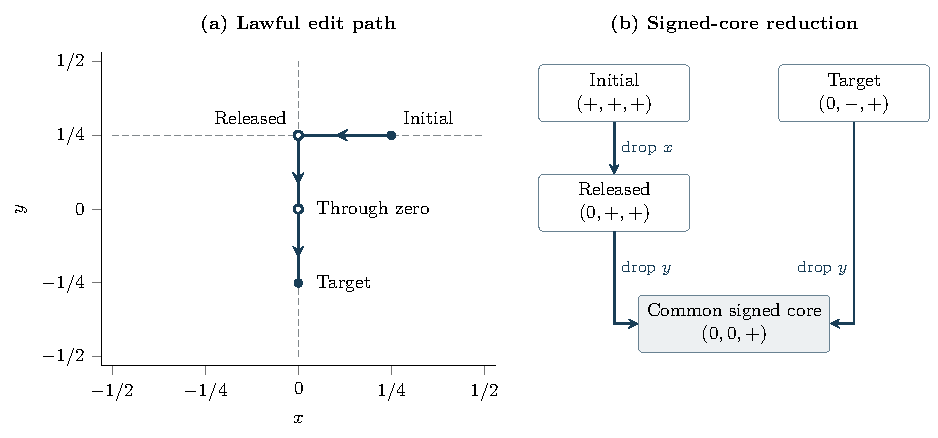
\includegraphics[width=\linewidth]{figures/signed_core_path.pdf}
 \caption{A lawful connection and its signed core at the same experimental
 profile. In (a), the dashed branches and the solid path together give
 the real lawful locus at \(z=1/4\) with the fourth response fixed at
 zero. The arrows trace the segments sampled by rational edits. The open
 circles are included intermediate states. In (b), the tuples give the
 signs of \(x,y,z\), and the arrows represent contractions. The initial
 law reaches the common signed core in two contractions and the target
 law reaches it in one. The calibration protects the positive sign at
 \(z\). Equality of the two signed cores is the reachability test at this
 fixed profile in \Cref{thm:native}.}
 \label{fig:staged-path}
\end{figure}

The support calculation behind this path is already instructive. A damping
weight specifies how many powers of a common parameter to multiply into each
response. As long as \(x,y,z\) are nonzero, the weight equations are
\(w_x+w_y=w_x+w_z\) and \(w_z=0\). They allow a contraction of \(x\) and force
\(y\) to survive. After \(x\) vanishes, the first equality is still true and
has zero on each side. It imposes no weight balance on the new support.
A second contraction can now remove \(y\). Both endpoints have the same signed
core, consisting of the positive calibrated \(z\). If the initial weight
equations were applied to every subsequent support, the initial positive
and target negative signs at \(y\) would stay distinct under all reductions.
This would incorrectly rule out \eqref{eq:opening-path}.

The geometric antecedent is the difference between a positive binomial
chart's closure and additional points of the full zero-allowing system.
Engstr\"om, Hersh and Sturmfels give an explicit example of that difference
in \emph{Toric Cubes}~\citep[Example~3]{toriccubes}.
The question here is whether such changes of active support admit a
\emph{complete} rational reachability criterion, and whether the criterion can
be recovered from actual held measurements. Sections~\ref{sec:spectral}
and~\ref{sec:native} address these two steps.

\subsection{Results and scope}

We first specify the measured model and the edit relation.
We then prove a separate theorem for bounded rational monomial systems.
It shows that a finite calculation on supports and signs captures every
real chart collision relevant to fine rational chains. The native theorem
combines it with homogeneous rate tests, conditional register constraints
and the order of attained profiles. The two complementary examples make
the criterion testable in both directions.

The lower-bound example uses the same coupled instrument for all six effects.
A subsequent classification of the available command families makes their
minimization precise. The terminal grade has a special role in the tests,
even when the command family takes the grade as an argument. We connect
these results to the witness predicates of Foundations~II in
\Cref{sec:witness-bridge}. The claims about reachability are specific to the
declared instruments, and the family count concerns the declared invocation
language.
